\documentclass{article}

\usepackage{here}
\usepackage{float}
\usepackage{adjustbox}
\usepackage{graphicx}
\usepackage{cite}
\usepackage{amsmath}
\usepackage{amssymb}
\usepackage{pifont}
\usepackage{enumitem}
\usepackage{url}
\usepackage{multirow}
\usepackage{etoolbox}
\usepackage{titlesec}
\usepackage{caption}
\captionsetup[table]{skip=5pt}
\newcommand{\cmark}{\ding{51}}

\DeclareMathOperator\erf{erf}

\interdisplaylinepenalty=2500
\hyphenation{op-tical net-works semi-conduc-tor}
\patchcmd{\thebibliography}{\section*{\refname}}{}{}{}
\setcounter{secnumdepth}{4}
\titleformat{\paragraph}
{\normalfont\normalsize\bfseries}{\theparagraph}{1em}{}
\titlespacing*{\paragraph}
{0pt}{3.25ex plus 1ex minus .2ex}{1.5ex plus .2ex}


\begin{document}

\title{The potential of a large dust grain in a collisionless plasma}
\author{Dogan Akpinar and George E. B. Doran}
\markboth{D. Akpinar \& G. E. B. Doran}
{Shell \MakeLowercase{\textit{et al.}}:}

\maketitle

\begin{abstract}
Abstract goes here
\end{abstract}

\section{Introduction}

\section{Background}

In the case of a large dust grain with a negative equilibrium charge, we can establish regions within an infinite plasma with well-defined
transitions. We firstly have the dust grain itself, followed
by a positive region of space, called the sheath, usually a few electron Debye lengths
in size. The electron Debye length is a characteristic length over which quasi-neutrality breaks down, 
defined as

\begin{equation}\label{eq:Debye}
\lambda_D = \sqrt{\frac{\varepsilon_{0} k_{B} T_{e}}{n_{0} e^2}},
\end{equation}

\medskip

\noindent where $k_B$ is the Boltzmann constant, $T_e$ is the electron temperature, $e$ is the 
electron charge, $n_0$ is the electron number density at infinity and $\varepsilon_{0}$ is the
permittivity of free space. Following the sheath, there exists the infinite pre-sheath where quasi-neutrality holds;
quasi-neutrality is mathematically written as an approximate equality between the ion and electron
densities, $Zn_i \approx n_e$.

\medskip

Positive ions are continuously collected by the negative dust, so there must be
a net influx of ions into the sheath to maintain the equilibrium. This establishes the Bohm
criterion, where the speed of ions required to enter the sheath must be 
greater then of equal to the Bohm speed. For the cold ion case, the Bohm speed is defined as

\smallskip 

\begin{equation}\label{eq:ColdBohm}
c_{s}^{cold} = \sqrt{\frac{k_{B}T_{e}}{m_{i}}},
\end{equation}

\noindent where $m_i$ is the ion mass and $c_{s}^{cold}$ is known as the cold ion Bohm speed. 
However, if we consider ions with a finite temperature, the required Bohm speed becomes 

\begin{equation}\label{eq:HotBohm}
c_{s}^{hot} = \sqrt{\frac{k_{B}(T_{e} + \gamma T_{i})}{m_{i}}},
\end{equation}

\smallskip

\noindent where $T_i$ is the ion temperature, $\gamma$ is the adiabatic index
and $c_{s}^{hot}$ is known as the hot ion Bohm speed \cite{Stangeby1986} \cite{Willis} .

\medskip

For a large dust grain, we may consider the planar sheath (thin sheath) limit \cite{Willis}. 
Hence, the potential drop across the sheath for $T_i \neq 0$ is given as

\begin{equation}\label{eq:SheathDrop}
\phi_s = \frac{k_B T_e}{2e}\ln{\left[\frac{2\pi Z^2}{\mu^2}(1 + \gamma \Theta)\right]},
\end{equation}

\noindent where $Z$ is the relative ion charge, $\mu = \sqrt{\frac{m_i}{m_e}}$ and $\Theta = \frac{T_i}{T_e}$ \cite{Stangeby1986}.

\section{Radial motion theory (ABR)}

\smallskip

The ABR model is a radial motion theory derived by Allen, Boyd and Reynolds. It describes the equilibrium surface potential acquired
by a dust grain immersed in an infinite and stationary plasma \cite{ABR}.

\medskip

Consider a spherical dust grain, of arbitrary radius $a$, immersed in this infinite plasma. Far from the surface we assume that the electron
and ion densities are equal, denoted $n_e$ and $n_i$ respectively; this is known as quasi-neutrality. As electrons are faster than ions, it can be shown that such a dust grain will become negatively 
charged \cite{Thomas}, thus ions will experience an attractive force due to the potential on the dust surface, 
$\phi_a$. We assume that ions at infinity have no kinetic energy, hence, they move radially
towards the dust grain. Therefore, it is appropriate to say that an ion at a distance 
$r$ from the dust center has radial speed $v_i$. Using energy conservation, one can show the following,

\begin{equation}\label{eq:EnergyConservation}
\frac{1}{2} m_i v_i^2 = -Ze\phi(r),
\end{equation}

\noindent where $\phi(r)$ is the potential at $r$, which vanishes as $r \to \infty$ \cite{ABR}.

\medskip

Equation (\ref{eq:EnergyConservation}) then leads to an expression for the ion current, which is entirely dependant on the radial distance from the 
dust grain, given by

\begin{equation}\label{eq:ABRIi}
I_i = \frac{4\sqrt{2} \ n_i \pi r^2 Z^{\frac{3}{2}}e^{\frac{3}{2}} \phi_a^{\frac{1}{2}} } {m_i^{\frac{1}{2}}}.
\end{equation}

As the potential is negative, few electrons reach the dust grain, hence, the electron density obeys a Boltzmann
distribution:

\begin{equation}\label{eq:ABRed}
n_e(r) = n_0 \exp{\left(\frac{e\phi(r)}{k_B T_e}\right)},
\end{equation}

\smallskip

we further assume that only inbound electrons contribute to the electron current at the surface of the dust
grain, given as

\begin{equation}\label{eq:ABRIe}
I_i = I_e = 4 \pi a^2 n_0 e \sqrt{\frac{k_B T_e}{2 \pi m_e }} \exp{\left(\frac{e \phi_a}{k_B T_e}\right)}.
\end{equation}  

\noindent where $m_e$ is the electron mass \cite{ABR}.

\medskip

It is useful to apply the following normalisations, noting that $\Phi$ is the opposite
sign for simplicity:

\begin{equation}\label{eq:ABRnorm}
{\Phi = - \frac{e\phi}{k_B T_e}}, \ {\rho = \frac{r}{\lambda_D}},\ {\alpha = \frac{a}{\lambda_D}},\ {J = \frac{I_i}{4 \pi \lambda_D^2 n_0 e \sqrt{\frac{2k_B T_e}{m_i}}}},
\end{equation}
    
\noindent where $\lambda_D$ is the electron Debye length, 

\medskip

Poisson's law allows for the formation of a differential equation which relates
the spatial variation of the potential to the difference in electron and 
ion densities,

\begin{equation}\label{eq:ABR9} 
\frac{d}{d\rho} \left(\rho^2 \frac{d\Phi}{d\rho}\right) = J Z^{-\frac{1}{2}}\Phi^{-\frac{1}{2}}  - \rho^2 \exp{(-\Phi)}.
\end{equation}

\medskip

\noindent This equation may be solved using the boundary conditions;

\begin{equation}\label{eq:ABR10}
\rho \approx J^{\frac{1}{2}} Z^{-\frac{1}{4}} \Phi^{-\frac{1}{4}} \exp{\left(\frac{\Phi}{2}\right)},
\end{equation}
 
\begin{equation}\label{eq:ABR11}
\frac{d\Phi}{d\rho}\biggr|_{\rho_b} = \frac{2\rho_b Z^{\frac{1}{2}} J^{-1} \Phi_b^{\frac{3}{2}}}{\Phi_b - \frac{1}{2}} exp{(-\Phi_b)},
\end{equation}
 
\begin{equation}\label{eq:ABR13}
\frac{J}{\Gamma} = \frac{4Z^{\frac{1}{2}}\Phi_b^{\frac{3}{2}}(2\Phi_b - 3)(2\Phi_b + 1)}{(2\Phi_b - 1)^3},
\end{equation}

\begin{equation}\label{eq:ABR12}
\frac{J}{\alpha^2} = \frac{\mu}{\sqrt{4\pi}} \exp{\left(-\Phi_a\right)},
\end{equation}

\medskip

\noindent which are formed by assuming that there exists a certain distance $\rho_b$, past which, quasi-neutrality applies. 
The potential at $\rho_b$ is given by $\Phi_b$, and $\Gamma$ is a number much greater than unity \cite{ABR}.
In order to find a value for the surface potential we must solve (\ref{eq:ABR9}), this may be 
achieved using a 4th order Runge-Kutta. We choose $\Gamma = 10000$ and find the roots of 
(\ref{eq:ABR13}) allowing us to determine the necessary boundary conditions 
using (\ref{eq:ABR10}) and (\ref{eq:ABR11}). Hence, solving the differential equation numerically, yields 
the following graph of normalised dust potential as a function of normalised dust radius.

\begin{figure}[H]
\centering
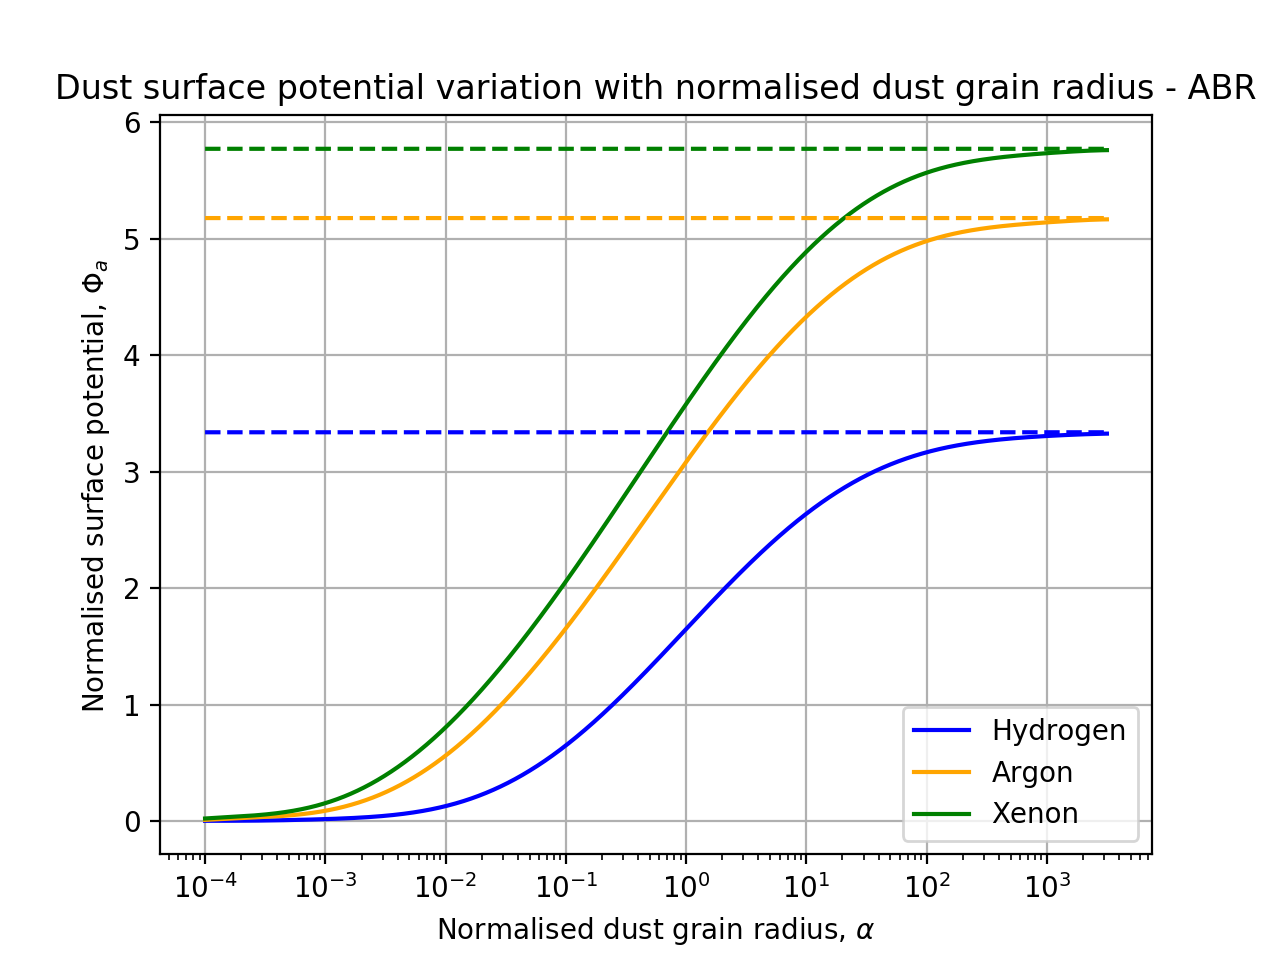
\includegraphics[width=\linewidth]{Output/ABRgraph.jpeg}
\caption{ABR predictions for $\Phi_a$ as a function of $\alpha$ for a dust grain in singly ionised Hydrogen, Argon and Xenon plasmas ($Z=1$) \cite{ABR} \cite{Thomas}.}
\label{ABR} 
\end{figure}

Thomas discusses that in the limit of $\alpha \to \infty$ the ABR potential approaches
the cold planar wall limit \cite{Thomas}, given as the following 

\begin{equation}\label{eq:ABRLim}
\lim_{\alpha \to \infty} \Phi_a = \frac{1}{2}\ln{\left(2 \pi \right)} - \frac{1}{2} - \ln{\left(\mu \right)},
\end{equation}

\smallskip

\noindent where $Z = 1$ and the $-\frac{1}{2}$ is due to the potential drop across the cold ion pre-sheath,
as discussed by Stangeby \cite{Stangeby1986} \cite{Stangeby2000}. Furthermore, one can clearly see that in the limit
of $\alpha \to 0$ the ABR prediction tends to zero also \cite{ABR}.

\section{Modified orbital motion limited (MOML)}

\smallskip

Orbital motion limited (OML) models the potential, $\phi_a$, on a small spherical
dust grain immersed in an infinite and collisionless plasma, it does so by considering
energy and angular momentum conservations of the ions along side a critical grazing incidence.
OML considers an equilibrium of ion and electron currents at the dust 
surface, $I_i = I_e$, while simultaneously invoking quasi-neutrality.
Hence, the standard result acquired from OML is 
the following

\begin{equation}\label{eq:OMLeqn}
\frac{\sqrt{\Theta}}{\mu} \left(1 - \frac{Z}{\Theta}\Phi_a \right) \approx \exp{\left(\Phi_a\right)},
\end{equation}

\smallskip

\noindent where $\Phi_a = \frac{e\phi_a}{k_B T_e}$.

\medskip

Using available OM data, Willis discusses that any error in OML is negligible for small dust grains,
he further proposes an upper radius limit for OML which is $\Theta$ dependant \cite{Willis}. Furthermore, it should be noted that
OML guarantees the existence of absorption radii, $r_{A} > a$, such that any 
ion within $r_{A}$ approaching the dust grain will be collected \cite{Thomas}. 

\medskip

In order to model a large dust grain, we must slightly change our approach to the problem.
We now apply OML to the boundary between the sheath and pre-sheath, this establishes
the assumption that as $\alpha \to \infty$ any ion that enters the sheath will be 
collected by the dust grain. For such dust grains, the majority of absorption
radii occur within the sheath, hence, applying OML in this was eliminates most of the inaccuracies introduced 
by absorption radii and ensures the validity of MOML. However, it will be shown later that the validity of MOML in fact breaks down for small
$\Theta$ \cite{Thomas}. 

\medskip

Replacing $\Phi_a$ on the left hand side in (\ref{eq:OMLeqn}) with $\Phi_s$, the normalised potential
at the sheath edge, physically amounts to
saying that as $\alpha \to \infty$, all ions that enter the sheath are absorbed. Considering an equilibrium of
electron and ion currents at the sheath edge while simultaneously invoking quasi-neutrality 
and the expression for the hot ion Bohm speed, (\ref{eq:HotBohm}), one acquires the following 
relationship between $\Phi_s$ and $\Phi_a$

\begin{equation}\label{eq:PhiS}
\Phi_s \approx \Phi_a - \frac{1}{2}\ln{\left[\frac{2\pi Z^2}{\mu^2}(1 + \gamma \Theta)\right]},
\end{equation}

\noindent where the second term is the normalised sheath potential drop, (\ref{eq:SheathDrop}).
Substituting (\ref{eq:PhiS}) into the modified (\ref{eq:OMLeqn}) and manipulating in terms of
the the principle branch of the Lambert W function, $W_0$, yields 

\begin{equation}\label{eq:MOMLsol}
\Phi_a =  \frac{\Theta}{Z} - W_{0}\left(\sqrt{2\pi \Theta (1 + \gamma \Theta)} \exp{\left (\frac{\Theta}{Z}\right)}\right) + \frac{1}{2}\ln{\left[\frac{2\pi Z^2}{\mu^2}(1 + \gamma \Theta)\right]}.
\end{equation}

Willis compares the MOML solution with simulated data ran by PIC and concludes that 
$\gamma = \frac{5}{3}$ seems to produce the most appropriate predictions \cite{Willis}. 
Hence, $\gamma = \frac{5}{3}$ is chosen as the default value for our investigation. It is worth noting
that from (Fig. \ref{MOMLgamma}) we see that for extreme, and even intermediate, $\Theta$ values, 
the choice of $\gamma$ has very little affect on the predicted potential.

\begin{figure}[H]
\centering
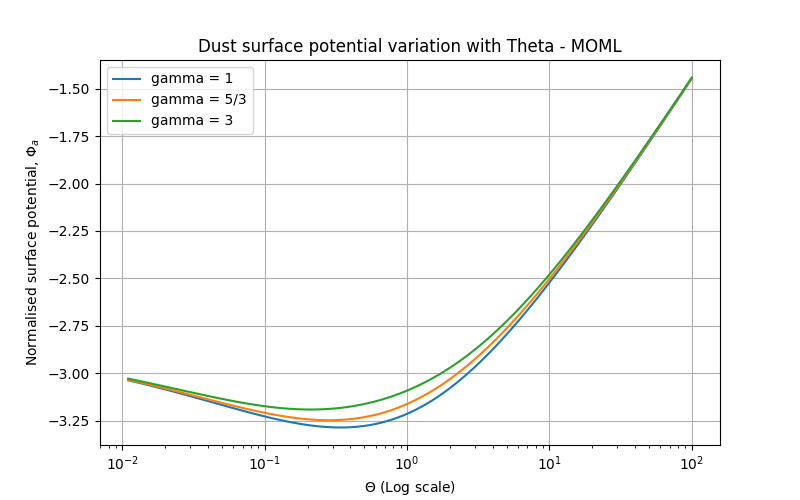
\includegraphics[width=\linewidth]{Output/MOMLgamma.jpeg}
\caption{The MOML prediction for  $\Phi_a$ as a function of $\Theta$, for a hydrogenic ($\mu \approx 43$) and singly ionised ($Z = 1$) plasma with different values of $\gamma$ \cite{Thomas}.}
\label{MOMLgamma} 
\end{figure}


\begin{figure}[H]
\centering
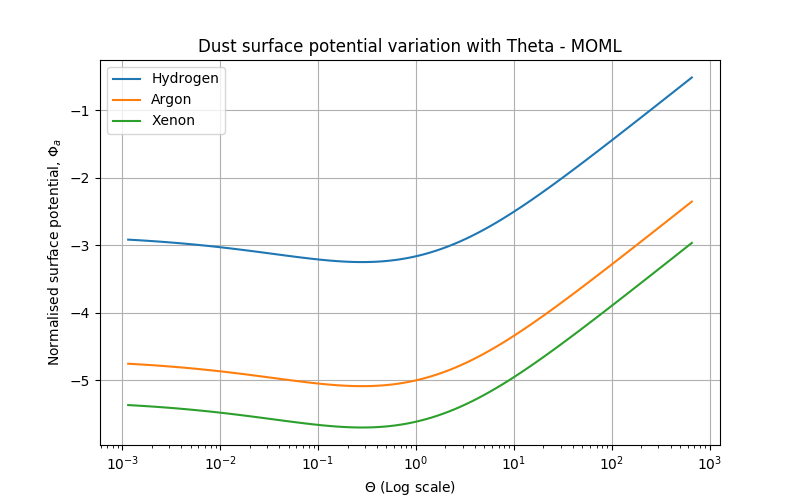
\includegraphics[width=\linewidth]{Output/MOMLgraph.jpeg}
\caption{Normalised surface potential as a function of $\Theta$ for singly ionised ($Z = 1$) Hydrogen, Argon and Xenon plasmas according on the MOML prediction, plotted on a log-linear scale.}
\label{MOMLgraph} 
\end{figure}
    
    
\section{SCEPTIC numerical fit}

\smallskip

SCEPTIC is used to investigate the charging of dust grains in a variety
of plasma conditions. Willis discusses that SCEPTIC data has been compared
to OM theory, and has shown that the agreement between the two is excellent over a large range of dust sizes 
for $\Theta = 0.01,0.1,1$ \cite{ScepticFit}.

\medskip

Upon further inspection of SCEPTIC data, Willis states that in the OML (small dust)
and planar sheath (large dust) limits, the (normalised) potential, $\Phi_a$, is independent of the (normalised)
dust radius, $\alpha$ \cite{ScepticFit}. He further states that the data in these cases can
be well fitted by the following expression

\begin{equation}\label{eq:SCEPTICfit}
\Phi_a = \lambda \ln{A} + \eta \ln{\Theta} + C,
\end{equation}

\smallskip

\noindent where A is the mass number of the ion species and $\lambda, \eta, C$ are 
constants. In this section we will only consider the SCEPTIC
fit for large dust grains; the following table summarises the values of $\lambda, \eta$ and $C$
for differing $\Theta$ ranges.

\begin{table}[h!]
\begin{center}
    \caption{SCEPTIC fit parameters for the planar sheath limit}
    \label{tab:ValueTable}
    \begin{tabular}{c|c|c|c} 
    \hline
    & $\lambda$ & $\eta$ & $C$ \\
    \hline
    $\Theta \leq 2$ & $0.456$ & $0$ & $3.179$\\
    $\Theta > 2$ & $0.557$ & $-0.386 - 0.024\ln{A}$ & $3.399$\\
    \end{tabular}
\end{center}
\end{table}


\section{Comparison between models for low $\Theta$}

\smallskip

It is well established that MOML agrees with SCEPTIC data, and by extension OM theory,
for finite $\Theta$ values. However, for values of $\Theta < 1$, MOML seems to breakdown and deviate 
from ABR and OM theory. 

\smallskip

Before explicitly comparing the models discussed until now, it should be noted that 
there is no available OM data for $\Theta < 0.01$, hence, we do not exactly know the predicted OM
values for a plasma with such conditions. This is entirely due to the complexity
of the theory itself and the limitation of numerical techniques available to solve its equations
with certainty. 

\smallskip

We may compare ABR and MOML in their respective limits to see if they are in 
agreement with one another, which is what we would expected.
If we consider ABR in the limit of $\alpha \to \infty$ we recover the cold planar
wall limit as shown in section 3, this value is approximately $-3.34$. If we now consider
the MOML solution, (\ref{eq:MOMLsol}) in the cold ion limit with $Z = 1$, we attain the following

\begin{equation}\label{eq:OMLLim}
\lim_{\Theta \to 0} \Phi_{a} = \frac{1}{2}\ln{\left(2 \pi \right)} - \ln{\left(\mu \right)}.
\end{equation}

\smallskip

This shows a discrepancy between ABR and MOML when MOML is used to
describe a cold ion plasma. As the ABR limit recovers well known and accepted values for
the potential drop across a cold plasma in the planar sheath limit \cite{Stangeby1986} \cite{Stangeby2000}, this results essentially
invalidates MOML in the cold ion limit.
    
\begin{figure}[H]
\centering
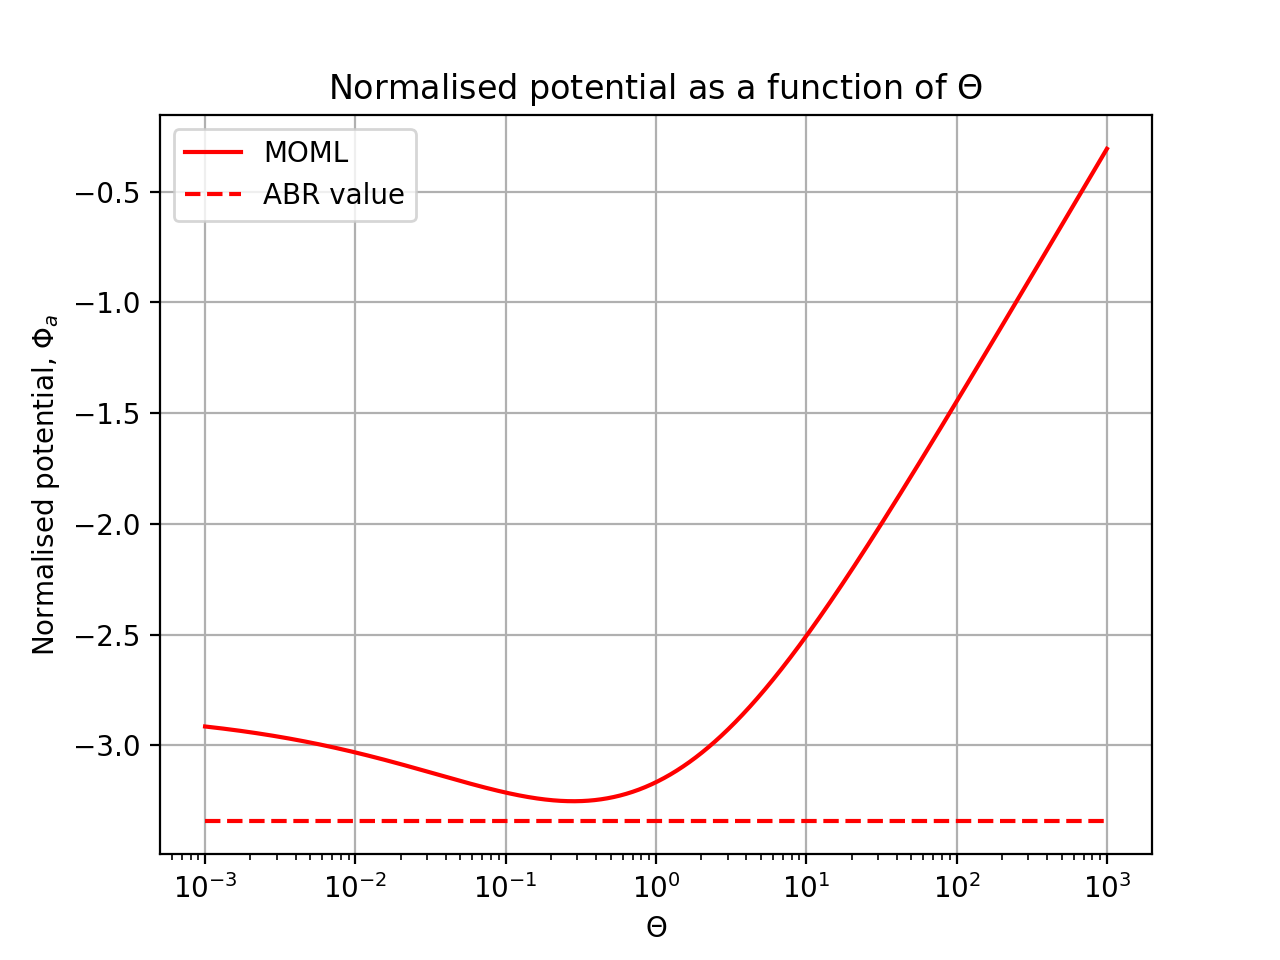
\includegraphics[width=\linewidth]{Output/MOMLvsABR.jpeg}
\caption{Normalised potential as a function of $\Theta$ for a singly charged hydrogenic plasma.
We in fact see that in the limit of $\Theta \to 0$ MOML does not agree with ABR.}
\label{MOMLvsABR} 
\end{figure}

Upon further investigation, one sees that in the cold ion limit, MOML
predicts a zero potential drop across the pre-sheath, where we expect it to be $-\frac{1}{2}$ \cite{Stangeby1986}.
It is believed that this discrepancy arises due to the existence of absorption radii well into
the pre-sheath for low $\Theta$, which is a result of applying OML at the sheath edge. 
Hence, we conclude that MOML is wrong for $\Theta \to 0$.

\section{Flowing sheath approximation}

We are now posed with the task of finding an analytic solution for the
potential on a large dust grain which is valid for low $\Theta$. The approach we will
take assumes the same electron behaviour as existing models \cite{Willis}, however, we wil slightly
change the behaviour of the ions to better suit the problem.

\smallskip

Our approach essentially considers each region of the plasma separately; we
already know an analytic solution for the potential drop across a planar sheath
for finite ion temperatures. However, in order to find the total potential drop across the plasma, we 
we must determine a temperature dependant potential drop across the pre-sheath.

\medskip 

We consider ions at infinity with an average energy of $E_0 = \kappa k_B T_i$, where
$\kappa$ is a constant to be determine. We now assume that the ions are modelled by a flowing 
Maxwellian at the sheath edge, with drift speed $u$,

\begin{equation}\label{FlowingMaxwellian}
f_i(\underline{\mathbf{v}}) = \left(\frac{m_i}{2\pi k_B T_i}\right)^{\frac{3}{2}} 
\exp{\left(\frac{-m_i}{2k_B T_i}|\underline{\mathbf{v}} - \underline{\mathbf{u}}|\right)}.
\end{equation}

\smallskip

In order to find the potential drop across the pre-sheath,
we must determine the average ion energy at the sheath edge, so we consider the following 
integral 

\begin{equation}\label{eq:Int1}
\langle E_{s} \rangle = \frac{1}{2}m_i \int v^2f_i(\underline{\mathbf{v}}) \,d^3 \underline{\mathbf{v}}.
\end{equation}

\smallskip
    
For convenience, we will drop the subscripts for the time being,
change to spherical polar coordinates and let $\xi = \frac{m}{2k_B T_i}$, yielding,

\begin{equation}\label{eq:Int2}
\langle E_{s} \rangle = \frac{1}{2}m \left(\frac{\xi}{\pi}\right)^{\frac{3}{2}}
\int v^4 \sin{\theta}\exp{\left(-\xi v^s - \xi u^2 + 2uv \xi \cos{\theta}\right)} \,dv d\theta d\phi,
\end{equation}

\noindent where $\theta$ and $\phi$ are the polar and azimuthal angle respectively. We continue
in the following way

\begin{equation}\label{eq:Int3}
\langle E_{s} \rangle = \pi m \left(\frac{\xi}{\pi}\right)^{\frac{3}{2}} \exp{\left(- \xi u^2\right)}
\int_{v = 0}^{\infty} v^4\exp{\left(-\xi v^2\right)} \int_{\theta = 0}^{\pi} \sin{\theta}\exp{\left(2uv \xi \cos{\theta}\right)} \,d\theta dv,
\end{equation}

\begin{equation}\label{eq:Int4}
\langle E_{s} \rangle = \frac{\pi m}{u\xi} \left(\frac{\xi}{\pi}\right)^{\frac{3}{2}} \exp{\left(- \xi u^2\right)}
\int_{v = 0}^{\infty} v^3\exp{\left(-\xi v^2\right)}\sinh{\left(2uv\xi\right)} \ dv,
\end{equation}

\noindent but

\begin{equation}\label{eq:Int5}
\int_{v = 0}^{\infty} v^3\exp{\left(-\xi v^2\right)}\sinh{\left(2uv\xi\right)} \ dv = \frac{u\sqrt{\pi}}{4\xi^{\frac{3}{2}}} 
\left(2\xi u^2 + 3\right) \exp{\left(\xi u^2\right)}.
\end{equation}

\smallskip

\noindent Substituting (\ref{eq:Int5}) into (\ref{eq:Int2}) yields the average energy 
in terms of $\xi$ and $u$ 

\begin{equation}\label{eq:AverageEnergy}
\langle E_{s} \rangle = \frac{1}{2}k_B T_i \left(2\xi u^2 + 3\right).
\end{equation}

Ions at the sheath edge must satisfy the hot ion Bohm criterion, $u \geq c_s^{hot}$. 
Choosing $u = c_s^{hot}$ amounts to saying that the average speed at the sheath edge 
is the hot ion Bohm speed. Hence, the average ion energy at the sheath becomes,

\begin{equation}\label{eq:AverageEnergy2}
\langle E_{s} \rangle = \frac{1}{2}k_B T_e \left(1 + \Theta\left(\gamma + 3\right)\right),
\end{equation}

\smallskip 

Using energy conservation across the pre-sheath,

\begin{equation}\label{eq:EnergyConservation2}
E_0 - \langle E_{s} \rangle = Ze\phi_p,
\end{equation}

\noindent then subbing in expressions for $E_0$, $\langle E_{s} \rangle$ and rearranging for $\phi$

\begin{equation}\label{eq:PS1}
Ze\phi_p = \kappa k_B T_i - \frac{1}{2}k_B T_e \left(1 + \Theta\left(\gamma + 3\right)\right),
\end{equation}
    
\noindent normalising yields,

\begin{equation}\label{eq:PSpotential}
\Phi_p =  - \frac{1}{2Z}\left(1 + \Theta\left(\gamma + 3 -2\kappa\right)\right),
\end{equation}

\smallskip

\noindent which is the temperature dependant pre-sheath potential drop.
When $\Theta = 0$ we recover the potential drop across a cold pre-sheath \cite{Stangeby1986}, 
which is very promising.

\smallskip

Therefore, we may determine the total potential drop across the plasma, by summing the known
$\Phi_s$ with the newly determined $\Phi_p$, given by the following equation

\begin{equation}\label{eq:FSpotential}
\Phi_a =  \frac{1}{2}\ln{\left[\frac{2\pi Z^2}{\mu^2}(1 + \gamma \Theta)\right]} - \frac{1}{2Z}\left(1 + \Theta\left(\gamma + 3 -2\kappa\right)\right),
\end{equation}

\medskip 

\noindent where $\gamma = \frac{5}{3}$ and $\kappa = 2$ give the best results. It should be noted 
that a possible justification for the optimal choice of $\kappa$ 
may be related to the ion heat flux \cite{Stangeby1986} \cite{Stangeby2000}.

\medskip

Figure (\ref{FSpotential}) shows the predicted dust potential as a function of $\Theta$ for 
our model; we see that for values of $\Theta \leq 1$ the potential seems reasonable, however, for higher
values of $\Theta$ the model seems to completely diverge from MOML. Initially, when seeing this behaviour 
one may become sceptical of our model, however, it should be noted that we have assumed that the average ion speed at
the sheath edge is equal to $c_s^{hot}$. It is very likely that the average ion
speed at the sheath edge is not $c_s^{hot}$, but in fact greater than $c_s^{hot}$. Hence, our assumption does not account for the possibility of the average ion 
speed being greater than $c_s^{hot}$. 

\medskip

In order to account for such a possibility, noting that our solution
for $\Phi_a$ is monotonically decreasing, we must consider that
$u \geq c_s^{hot}$, yielding a lower bound for the average ion energy at the sheath edge

\begin{equation}\label{eq:AverageEnergy}
\langle E_{s} \rangle \geq \frac{1}{2}k_B T_i \left(2\xi u^2 + 3\right).
\end{equation}

\medskip

Following the same steps as (\ref{eq:AverageEnergy2}) through (\ref{eq:PSpotential}) we determine that

\begin{equation}\label{eq:LowerBound}
\Phi_a \geq  \frac{1}{2}\ln{\left[\frac{2\pi Z^2}{\mu^2}(1 + \gamma \Theta)\right]} - \frac{1}{2Z}\left(1 + \Theta\left(\gamma + 3 -2\kappa\right)\right),
\end{equation}

\noindent suggesting that the potential predicted by this model acts as a lower bound for the dust grain potential.

\begin{figure}[H]
\centering
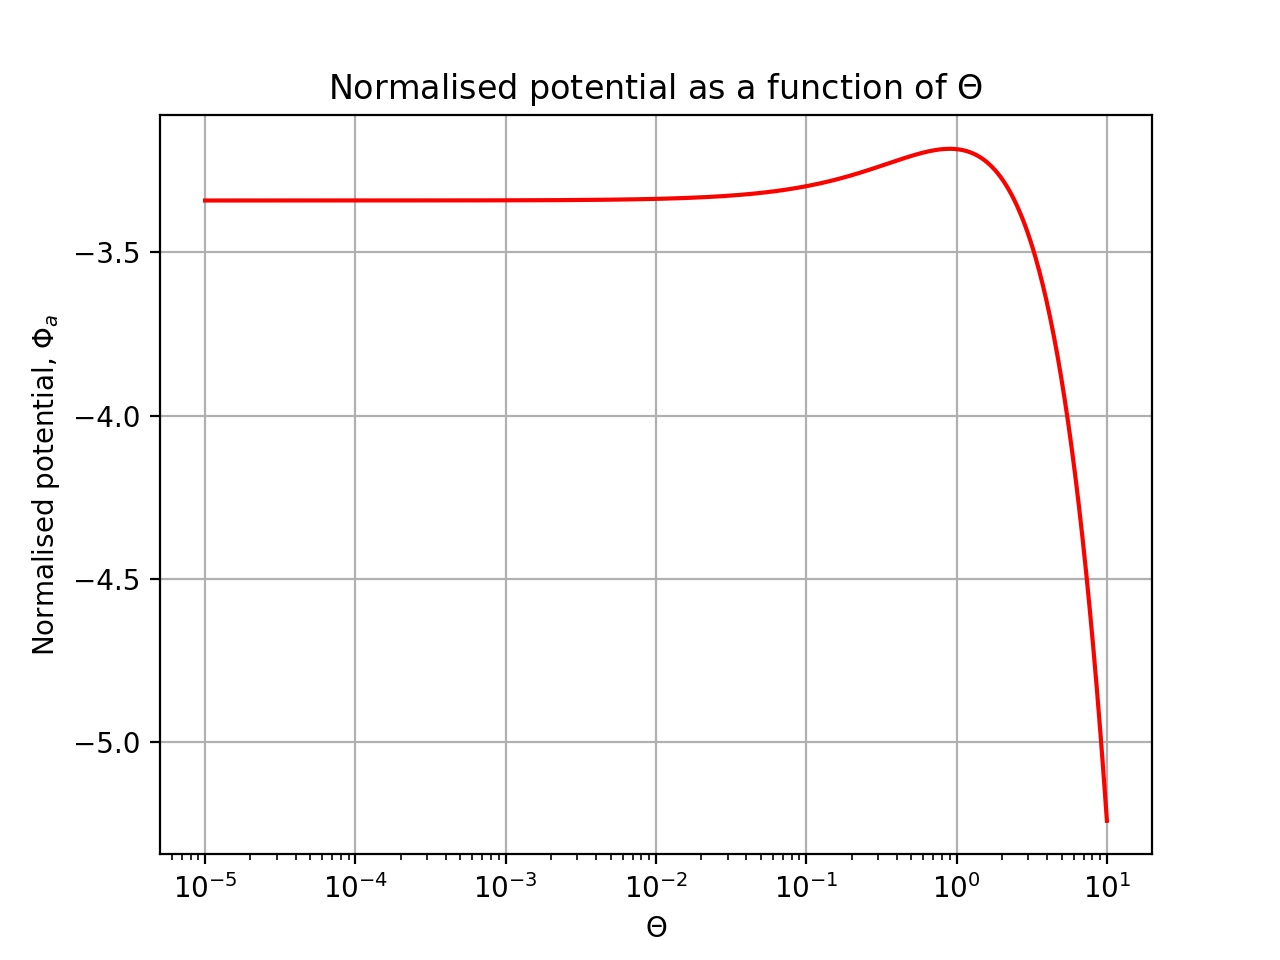
\includegraphics[width=\linewidth]{Output/FSpotential.jpeg}
\caption{Normalised potential as a function of $\Theta$ for a singly charged hydrogenic plasma
using our newly determined model.}
\label{FSpotential} 
\end{figure}

\subsection{Validity range for our model}

\smallskip

In order to determine the reliability of our model, we must compare it to existing 
models that are accepted within the plasma community. As stated before, we know that 
our new model deviates from MOML for values of $\Theta > 1$; however, the MOML potential 
is in fact greater than the potential predicted by model in this region, and so is above
the lower bound that our model imposes. Therefore, for values of $\Theta > 1$, MOML is still the most
appropriate model available. 

\medskip

The most interesting behaviour of our model is seen for $\Theta \leq 1$. In the limit of 
$\Theta \to 0$ our model exactly recovers the ABR value and so rectifies the discrepancy between
MOML and ABR. Furthermore, the value predicted by the flowing sheath approximation for 
$\Theta = 1$ is the same as that predicted by OM theory for $\alpha = 1$ and $\Theta = 1$, suggesting 
that our model exactly reproduces known values for the extreme values of $0 \leq \Theta \leq 1$.
Within the region of interest, we see that our model predicts an 
increasing potential from the ABR value, as is expected, in direct contrast to a decreasing potential from a 
wrong cold ion value as suggested by MOML.

\begin{figure}[H]
\centering
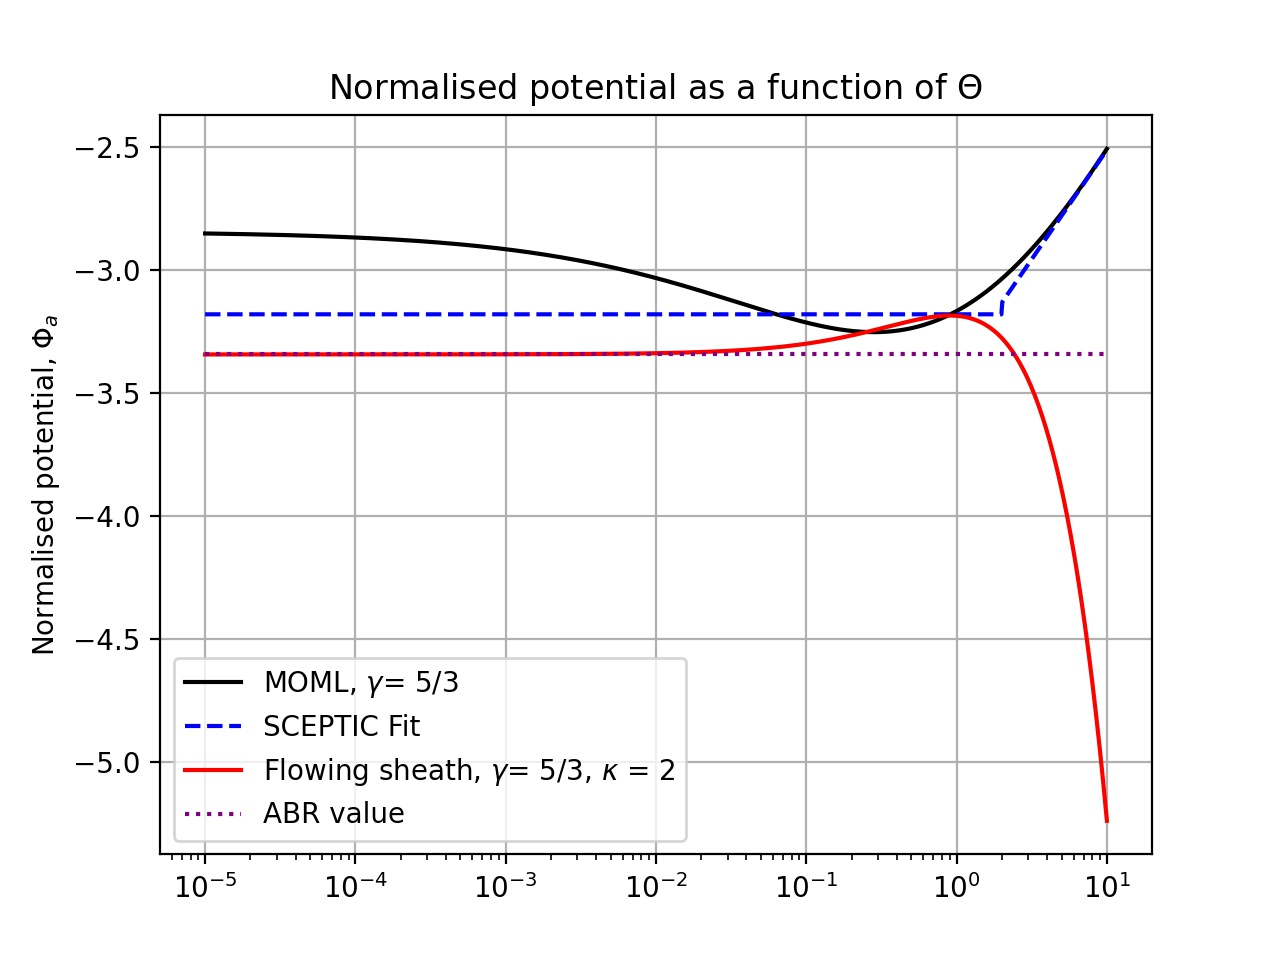
\includegraphics[width=\linewidth]{Output/ModelComparions.jpeg}
\caption{Normalised potential as a function of $\Theta$ for a singly charged hydrogenic plasma using MOML, SCEPTIC,
ABR and the flowing sheath approximation.}
\label{ModelComparions} 
\end{figure}

Upon further analysis, as shown in figure (\ref{MOMLvsFS}), we have determined 
that in this range the flowing sheath approximation has, on average, 
a smaller percentage difference from the SCEPTIC fit. Therefore, If we assume
the SCEPTIC fit to be correct for $\Theta \to 0$, ignoring its discrepancy from ABR, we find that the
flowing sheath approximation is the better model in this range. Thus providing sufficient evidence to replace MOML with 
the flowing sheath approximation for these values of $\Theta$.

Therefore, the new proposed potential on a large dust grain in a finite temperature plasma is given as follows

\begin{equation}
\Phi_a = 
\begin{cases}
\frac{1}{2}\ln{\left[\frac{2\pi Z^2}{\mu^2}(1 + \gamma \Theta)\right]} - \frac{1}{2Z}\left(1 + \Theta\left(\gamma + 3 -2\kappa\right)\right) & \text{for }0 \leq \Theta \leq 1\\
\frac{\Theta}{Z} - W_{0}\left(\sqrt{2\pi \Theta (1 + \gamma \Theta)} \exp{\left (\frac{\Theta}{Z}\right)}\right) + \frac{1}{2}\ln{\left[\frac{2\pi Z^2}{\mu^2}(1 + \gamma \Theta)\right]} & \text{for } \Theta > 1
\end{cases}
\end{equation}

\noindent where $\gamma = \frac{5}{3}$ and $\kappa = 2$ give the best results.

\begin{figure}[H]
\centering
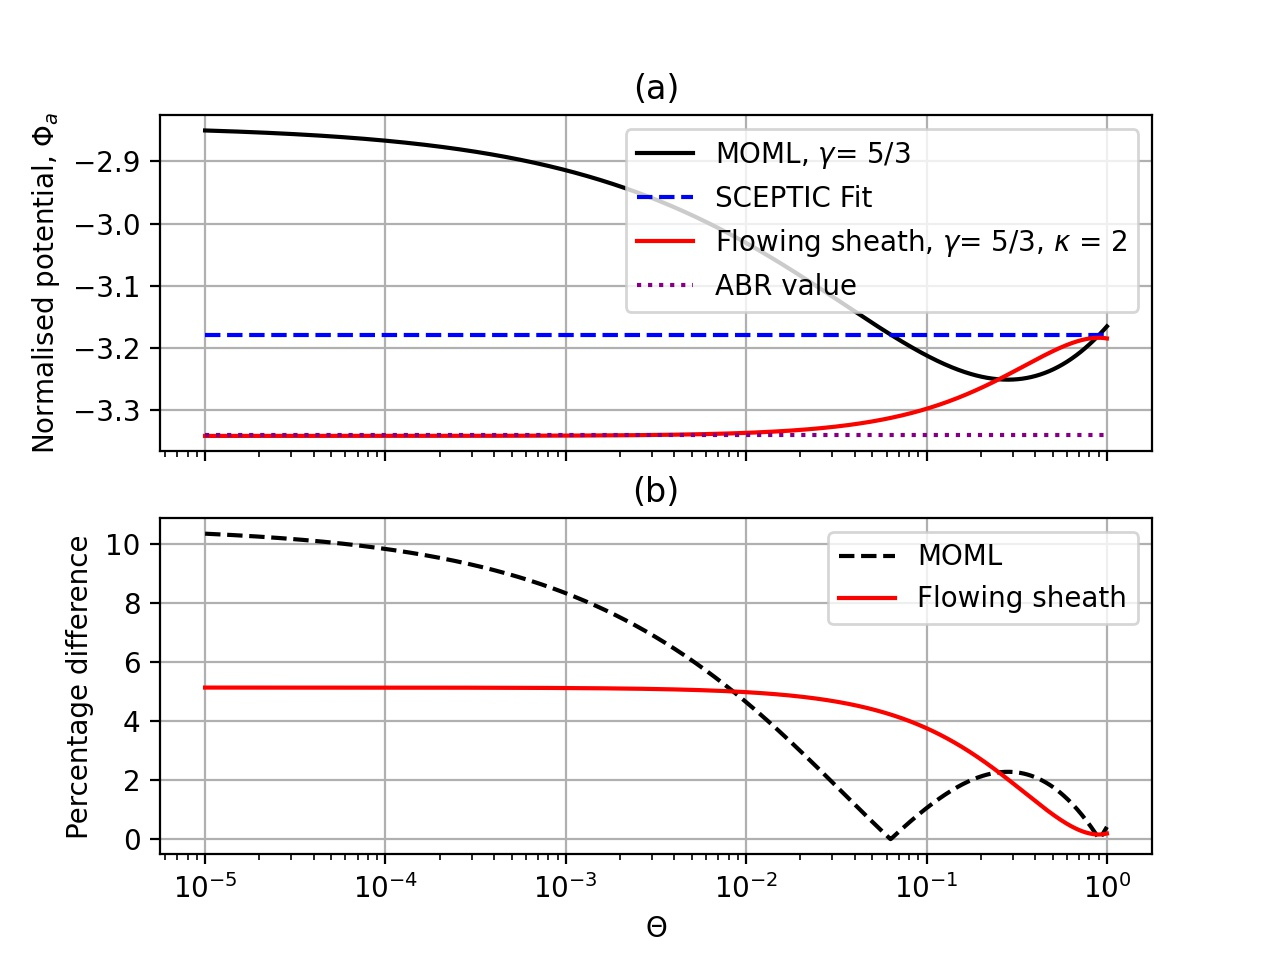
\includegraphics[width=\linewidth]{Output/MOMLvsFS.jpeg}
\caption{(a) Variation of normalised potential with $\Theta$ for a singly charged hydrogenic plasma using MOML, SCEPTIC,
ABR and the flowing sheath approximation. (b) Percentage difference between MOML, flowing 
sheath approximation and the SCEPTIC fit.}
\label{MOMLvsFS} 
\end{figure}

\section{Conclusion}


\section{References and Acknowledgements}
\bibliography{DustyLib}
\bibliographystyle{IEEEtran}

\section{Appendix}

\subsection{Symbol dictionary}
\begin{center}
\begin{tabular}{cl} 

$e$ & Electron charge \\
$\varepsilon_0$ & Permittivity of free space \\
$k_B$ & Boltzmann's constant \\
$a$ & Dust radius\\
$\alpha$ & Normalised dust radius \\
$_a$ & Subscript indicating a quantity at the dust grain surface \\
$r$ & Distance from the centre of the dust grain \\
$\rho$ & Normalised distance from the centre of the dust grain \\
$\lambda_D$ & Debye length \\
$m_j$ & Mass \\
$n_j$ & Density \\
$T_j$ & Temperature \\
$I_j$ & Current \\
$_j$ & Subscript indicating a plasma particle \\
$_i$ & Subscript indicating an ion quantity \\
$_e$ & Subscript indicating an electron quantity \\
$_0$ & Subscript indicating an electron quantity at infinity \\
$\mu$ & Root mass ratio\\
$\Theta$ & Ratio of ion to electron temperature \\
$\gamma$ & Heat capacity ratio \\
$u$ & Flow velocity \\
$\upsilon$ & Normalised flow velocity \\
$\Gamma$ & ABR correction factor \\
$Z$ & Ion charge number \\
$Q$ & Dust grain charge \\
$\phi$ & Electric potential \\
$\Phi$ & Normalised electric potential \\

\end{tabular}
\end{center}



\end{document}